\chapter{System Implementation}

% In this section, we present the technology stack that will be used and the implementation as well as the result of each component of the system.

\section{Technology Stack}

\subsection{Programming Language}
\subsubsection{HTML, CSS, Javascript}
HTML (HyperText Markup Language), CSS (Cascading Style Sheets), and Javascript are the three core technologies of the web development field. 
\begin{itemize}

    \item \textbf{HTML (Hyper Text Markup Language)} is used to define the structure of a web page. Every web page consists of a set of HTML elements. Each HTML element is represented by a tag. The web browser reads the HTML tags from top to bottom and renders the web page accordingly.

    \item \textbf{CSS (Cascading Style Sheets)}: the language for defining the style of a web page. CSS is used to define the position, size, color, font, etc of the HTML elements. With the help of HTML and CSS, we can build a beautiful and responsive static web page. 

    \item \textbf{JavaScript} is a scripting or programming language that allows you to implement complex features on web pages. With Javascript, we can add the dynamic behavior of the web page. For example, we can use Javascript to validate the form, change the content of the web page, handle user's input etc.
\end{itemize}

\begin{figure}[ht]
    \centering
    
\includegraphics[width=0.5\textwidth]{../Images/8.Technology_Stack/html_css_js.png}
    \caption{HTML, CSS, and Javascript}
    \label{fig:html_css_javascript}
\end{figure}

\subsubsection{Python}
\textbf{Python} is an easy-to-learn and powerful programming language. It was created by Guido van Rossum. Python is designed to be a general-purpose language, which means that it can be applied in a wide range of domains such as web development, data science, machine learning, etc. In the process of developing the project, our group chose Python 3.11 as the main programming language to build machine learning models and the API server. The reasons for choosing Python are:
\begin{itemize}
    \item Python with clean and simple syntax is easy to learn and use. When developing the application with Python, we can focus on the core idea of the application instead of worrying about the syntax.
    \item Python has a large community and a huge number of libraries, especially in the field of machine learning and web development. Some popular libraries are NumPy, Pandas, Scikit-learn, TensorFlow, PyTorch, etc.
\end{itemize}

\begin{figure}[ht]
    \centering
    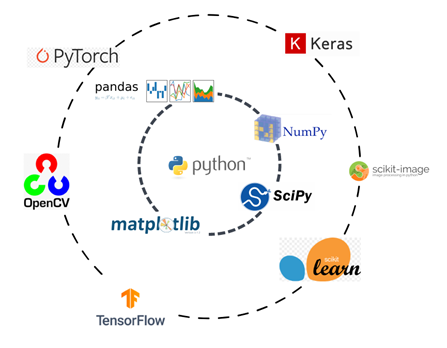
\includegraphics[width=0.6\textwidth]{../Images/8.Technology_Stack/python_ecosystem.png}
    \caption{The Python Ecosystem in Machine Learning}
    \label{fig:python_ecosystem}
\end{figure}



\subsection{Libraries and Frameworks}
\subsubsection{Scrapy}
Scrapy is a free and open-source Python framework for web scraping. It provides a simple API for crawling the data from the web page. Scrapy is built on top of Twisted, an asynchronous networking framework. Scrapy is a powerful tool for web scraping. It can be used to automate the process of crawling data from the web page. In this project, we use Scrapy to crawl the rental data from real estate websites.
\begin{figure}[ht]
    \centering
    
\includegraphics[width=0.5\textwidth]{../Images/8.Technology_Stack/scrapy.png}
    \caption{Scrapy}
    \label{fig:scrapy}
\end{figure}

\subsubsection{Puppeteer}
In our project, we need to crawl the data from Facebook pages. Facebook is a client-side rendered website, which means that the HTML content is generated by Javascript. A Scrapy spider cannot crawl the data from Facebook pages because it just downloads and parses the HTML content to get the data. However, with client-side rendered websites like Facebook, the HTML content does not contain the data that we need. Therefore, we need to use a tool that can execute the Javascript code to get the data. In this case, Puppeteer is a good choice. Puppeteer is a powerful tool for web scraping. The advantage of Puppeteer is that it can execute the Javascript code and get the data from the client-side rendered websites. In our project, we use Puppeteer to crawl the data from Facebook pages.

\begin{figure}[ht]
    \centering 
    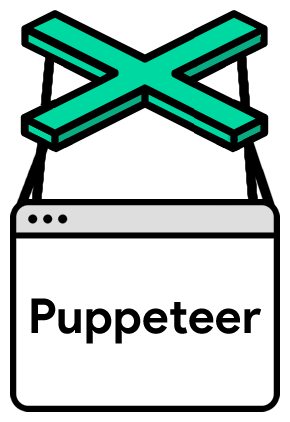
\includegraphics[height=0.2\textheight]{../Images/8.Technology_Stack/puppeteer.png}
\end{figure}

\subsubsection{React and Next.js}
\textbf{React} is the JavaScript library developed by Facebook for building user interfaces. React is a component-based library. It means that a React application is built from a set of encapsulated components. Each component is a reusable piece of code that can represent both a part of the user interface and its logic. React library helps developers to build a large and complex user interface simply. However, React is just a UI library, it missing some tools for building a complete web application such as routing, server-side rendering and state management. Therefore, when working with React, we need to use other libraries to extend its functionality. 

For these reasons, we use \textbf{NextJS} to build the web application. NextJS is a framework built on top of React, so NextJS has all the features of React and also provides some useful features such as routing and server-side rendering. Using NextJS helps us reduce the amount of time to set up the project and also takes advantage of server-side rendering to improve the performance of the web application.

\begin{figure}[ht]
    \centering
    \begin{subfigure}{0.4\textwidth}
        \centering
        
\includegraphics[width=0.7\textwidth]{Images/8.Technology_Stack/react_logo.png}
        \caption{React}
    \end{subfigure}
    \begin{subfigure}{0.4\textwidth}
        \centering
        
\includegraphics[width=\textwidth]{Images/8.Technology_Stack/nextjs_logo.png}
        \caption{NextJS}
    \end{subfigure}
\end{figure}

\subsubsection{FastAPI}
FastAPI is a modern, fast (high-performance), web framework for building APIs with Python. FastAPI is one of the most popular web frameworks for building APIs in Python. FastAPI provides some useful features such as \cite{fastapi}:
\begin{itemize}
    \item FastAPI is easy to learn and use. It has a simple and clean syntax.
    \item FastAPI is fast. It is built on top of Starlette and Pydantic, so it has high performance.
    \item Fast to code: FastAPI has a simple and intuitive API, so we can build the API quickly.
    \item Fewer bugs: Reduce about 40\% of human (developer) induced errors
\end{itemize} 

\noindent Within the scope of our project, we use FastAPI to build the API server for the AI services. 

\begin{figure}[ht]
    \centering
    
\includegraphics[width=0.5\textwidth]{../Images/8.Technology_Stack/fastapi_logo.png}
    \caption{FastAPI}
    \label{fig:fastapi}
\end{figure}

\subsubsection{NodeJS and Express}
\textbf{NodeJS} is an open-source, cross-platform, JavaScript runtime environment that executes JavaScript code outside a web browser. NodeJS is built on top of the V8 engine, which is the open-source JavaScript engine that runs in Google Chrome and other Chromium-based web browsers. NodeJS allows developers to use JavaScript to build the backend of the web application.
\begin{figure}[ht]
    \centering
    
\includegraphics[width=0.5\textwidth]{../Images/8.Technology_Stack/nodejs_logo.png}
    \caption{NodeJS, Source: \cite{nodejs}}
    \label{fig:nodejs}
\end{figure}

\textbf{Express} is a minimal and flexible Node.js web application framework that provides a robust set of features for web and mobile applications. Express is the most popular NodeJS framework. It provides some useful features such as routing, middleware, etc. In our project, we use Express to build the API server for the rental service.

\subsubsection{MongoDB}
MongoDB is a document-oriented database. It stores the data in the form of documents. Each document is a set of key-value pairs. MongoDB is a NoSQL database, so it does not require a predefined schema. The reason for choosing MongoDB is the flexibility. Our data is crawled from different sources, so the data does not have a fixed schema. Therefore, using MongoDB helps us store the data easily.

Besides, MongoDB has a cloud version called MongoDB Atlas. MongoDB Atlas is a fully managed cloud database. It provides us with a simple way to deploy, operate, and scale the MongoDB database in the cloud. In our project, we use MongoDB Atlas to store the data.

\begin{figure}[ht]
    \centering
    
\includegraphics[width=0.5\textwidth]{../Images/8.Technology_Stack/mongodb_logo.png}
    \caption{MongoDB}
    \label{fig:mongodb}
\end{figure}


\subsubsection{Pandas}
Pandas is a Python library for data manipulation and analysis. It provides simple and powerful functions to manipulate the data. In our project, we use Pandas to preprocess the data before feeding it to the machine learning model.

\begin{figure}[ht]
    \centering
    
\includegraphics[width=0.5\textwidth]{../Images/8.Technology_Stack/pandas_logo.png}
    \caption{Pandas}
    \label{fig:pandas} 
\end{figure}

\subsubsection{Matplotlib}
Matplotlib is a comprehensive library for creating static, animated, and interactive visualizations in Python. With Matplotlib, we can create many types of charts such as line charts, bar charts, pie charts, etc. Using Matplotlib helps us visualize the data and understand the data better.

\begin{figure}[ht]
    \centering
    
\includegraphics[width=0.5\textwidth]{../Images/8.Technology_Stack/matplotlib_logo.png}
    \caption{Matplotlib}
    \label{fig:matplotlib}
\end{figure}

\subsubsection{Pytorch}
Pytorch is an open-source machine learning framework based on the Python programming language and the Torch library. It is used in many fields in machine learning such as Computer Vision and Natural language processing.  Pytorch provides some features that help us build the machine learning models easily such as:
\begin{itemize}
    \item Tensor computation with strong GPU acceleration. It helps us take advantage of GPU to speed up the training process.
    \item Automatic differentiation: As we know building the machine learning model requires the forward and backward propagation process. With Pytorch, we just need to define the forward propagation process, Pytorch will automatically compute the backward propagation process and update the parameters of the model.
    \item Pytorch provides many useful libraries for building the machine learning model and is compatible with other popular libraries such as Numpy and Pandas.
\end{itemize}

\noindent Besides these useful features, Pytorch is open-source and has a strong community. For these reasons, we choose Pytorch to build machine-learning models for the intent classifier and entity extractor.

\begin{figure}[ht]
    \centering
    
\includegraphics[width=0.5\textwidth]{../Images/8.Technology_Stack/pytorch_logo.png}
    \caption{Pytorch}
    \label{fig:pytorch}
\end{figure}

\subsubsection{Transformers}
Transformers provides APIs and tools to easily download and train state-of-the-art pre-trained models. These pre-trained models support common tasks in different modalities such as Natural Language Processing (NLP), Computer Vision (CV) and Speech Recognition (ASR). After training the model, Transformers also provides a way to share the model with the community on the Hugging Face Hub. The Hub now has more than 120k models, 20k datasets and 50k demos. This is a central place where anyone can share, explore, discover and experiment with open-source Machine Learning \cite{huggingface}.

\begin{figure}[ht]
    \centering
    
\includegraphics[width=0.5\textwidth]{../Images/8.Technology_Stack/huggingface_logo.png}
    \caption{Hugging Face}
    \label{fig:huggingface}
\end{figure}

\subsubsection{PhoBERT}
PhoBERT is the pre-trained language model for Vietnamese. PhoBERT is trained on a large corpus of Vietnamese text data with more than 20GB of Wikipedia and News text. PhoBERT is compatible with the Transformers library, so we can easily download and use the pre-trained model from the Hugging Face Hub. In our project, we use PhoBERT in our machine learning models \cite{phobert}.

\subsection{Tools}

\subsubsection{Git and GitHub}
\textbf{Git} is a distributed version control system. Using Git helps us manage the source code of the project easily. Git provides many useful features such as branching, merging, and tagging. With these features, Git allows developers to work on the same project at the same time without worrying about conflicts. Git is also a cross-platform tool, so we can use it on many operating systems such as Windows, Linux, and macOS.

\begin{figure}[ht]
    \centering
    
\includegraphics[width=0.5\textwidth]{../Images/8.Technology_Stack/git_logo.png}
    \caption{Git}
    \label{fig:git}
\end{figure}

\noindent \textbf{GitHub} is a platform for hosting and collaborating on Git repositories. GitHub allows developers to store the source code on the cloud and collaborate with other developers.

\begin{figure}[ht]
    \centering
    
\includegraphics[width=0.5\textwidth]{../Images/8.Technology_Stack/github_logo.png}
    \caption{GitHub}
    \label{fig:github}
\end{figure}

\subsubsection{Github Actions}
GitHub actions is a CI/CD tool provided by GitHub. It helps us automate the process of building, testing, and deploying the application. With GitHub actions, we can easily set up the CI/CD pipeline for the project. In our project, we use GitHub actions to build and deploy the web application to the server.

\subsubsection{Dagshub}
With GitHub, developers can only manage their source code. But in the machine learning project, we also need to manage the data and the model. So \textbf{Dagshub} appears to solve this problem.
Dagshub is a platform for developers to manage their machine-learning projects. Dagshub is built on top of Git, so it has all the features of Git. Besides, Dagshub also provides some useful features for managing the data and the model.

\begin{figure}[ht]
    \centering
    
\includegraphics[width=0.5\textwidth]{../Images/8.Technology_Stack/dagshub_logo.png}
    \caption{Dagshub}
    \label{fig:dagshub}
\end{figure}

\section{Implementation and Results}
In this chapter, we present the process of implementing the system. Up to the end of the Specialized Project, we have completed the following tasks:
\begin{itemize}
    \item Designed a mockup interface for the website.
    \item Developed a crawler to collect data from both real estate websites and Facebook groups.
    \item Developed an intent classification model to classify the user's intent based on the user's message.
\end{itemize}

\subsection{Mockup interface}
We have implemented the mockup interface in Figma for the Tenant Landing Page, Search page, Rental detail page and Chatbot interface. All of the mockup interfaces are in \href{https://www.figma.com/proto/4W6eMgIgZQaSfi5h8Mn8Af/Material-UI-for-Figma-(and-MUI-X)-(Community)-(Copy)?page-id=4230%3A722&type=design&node-id=6609-8548&viewport=4481%2C1065%2C1&t=QoVk3s8CM7w3qcvh-1&scaling=scale-down-width&starting-point-node-id=6759%3A76810}{here}

\subsubsection{Tenant pages}
We have a tenant landing page that allows the user to view the list of rental posts in the system. You can see the design in Figure \ref{fig:tenant-landing-page}

\clearpage
\begin{figure}[ht]
    \centering
    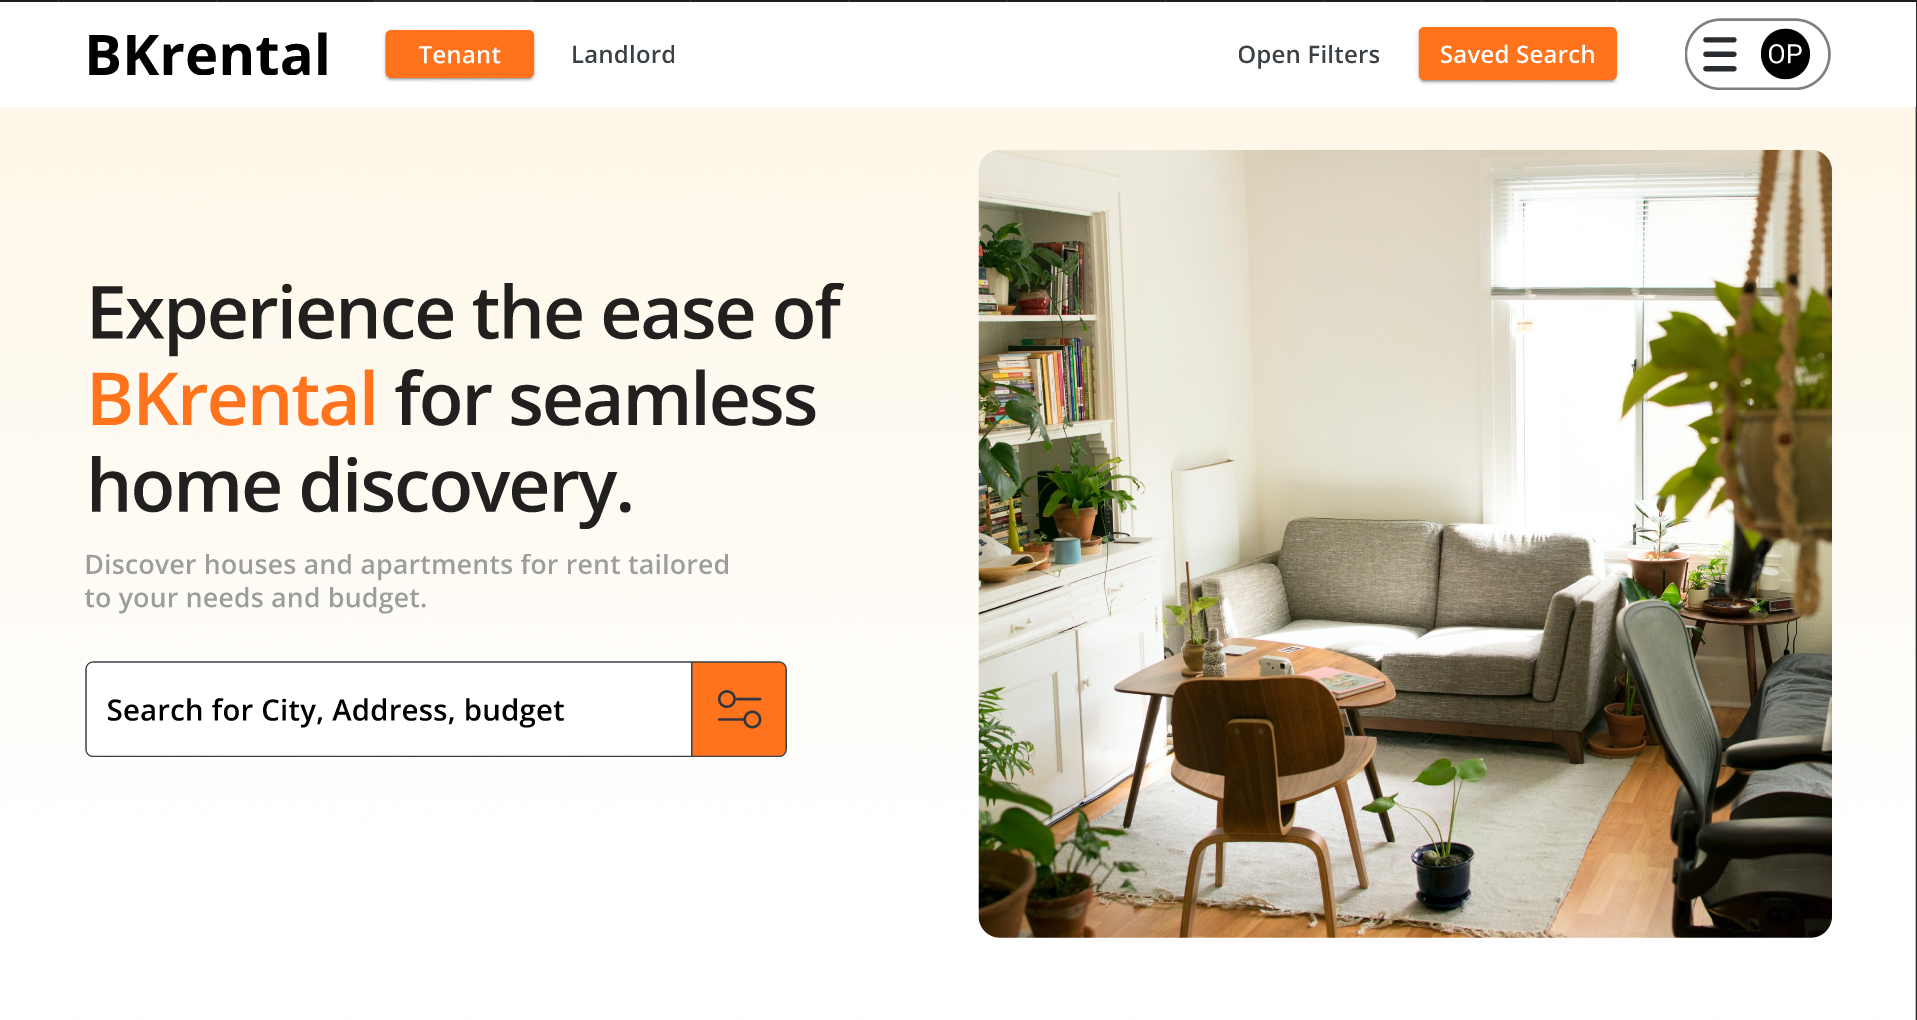
\includegraphics[width=0.8\textwidth]{Images/Mockup/landing_page.png}
    \caption{The tenant landing page}
    \label{fig:tenant-landing-page}
\end{figure}

The list of rental posts is displayed in the form of a card, see Figure \ref{fig:rental-posts}

\begin{figure}[ht]
    \centering
    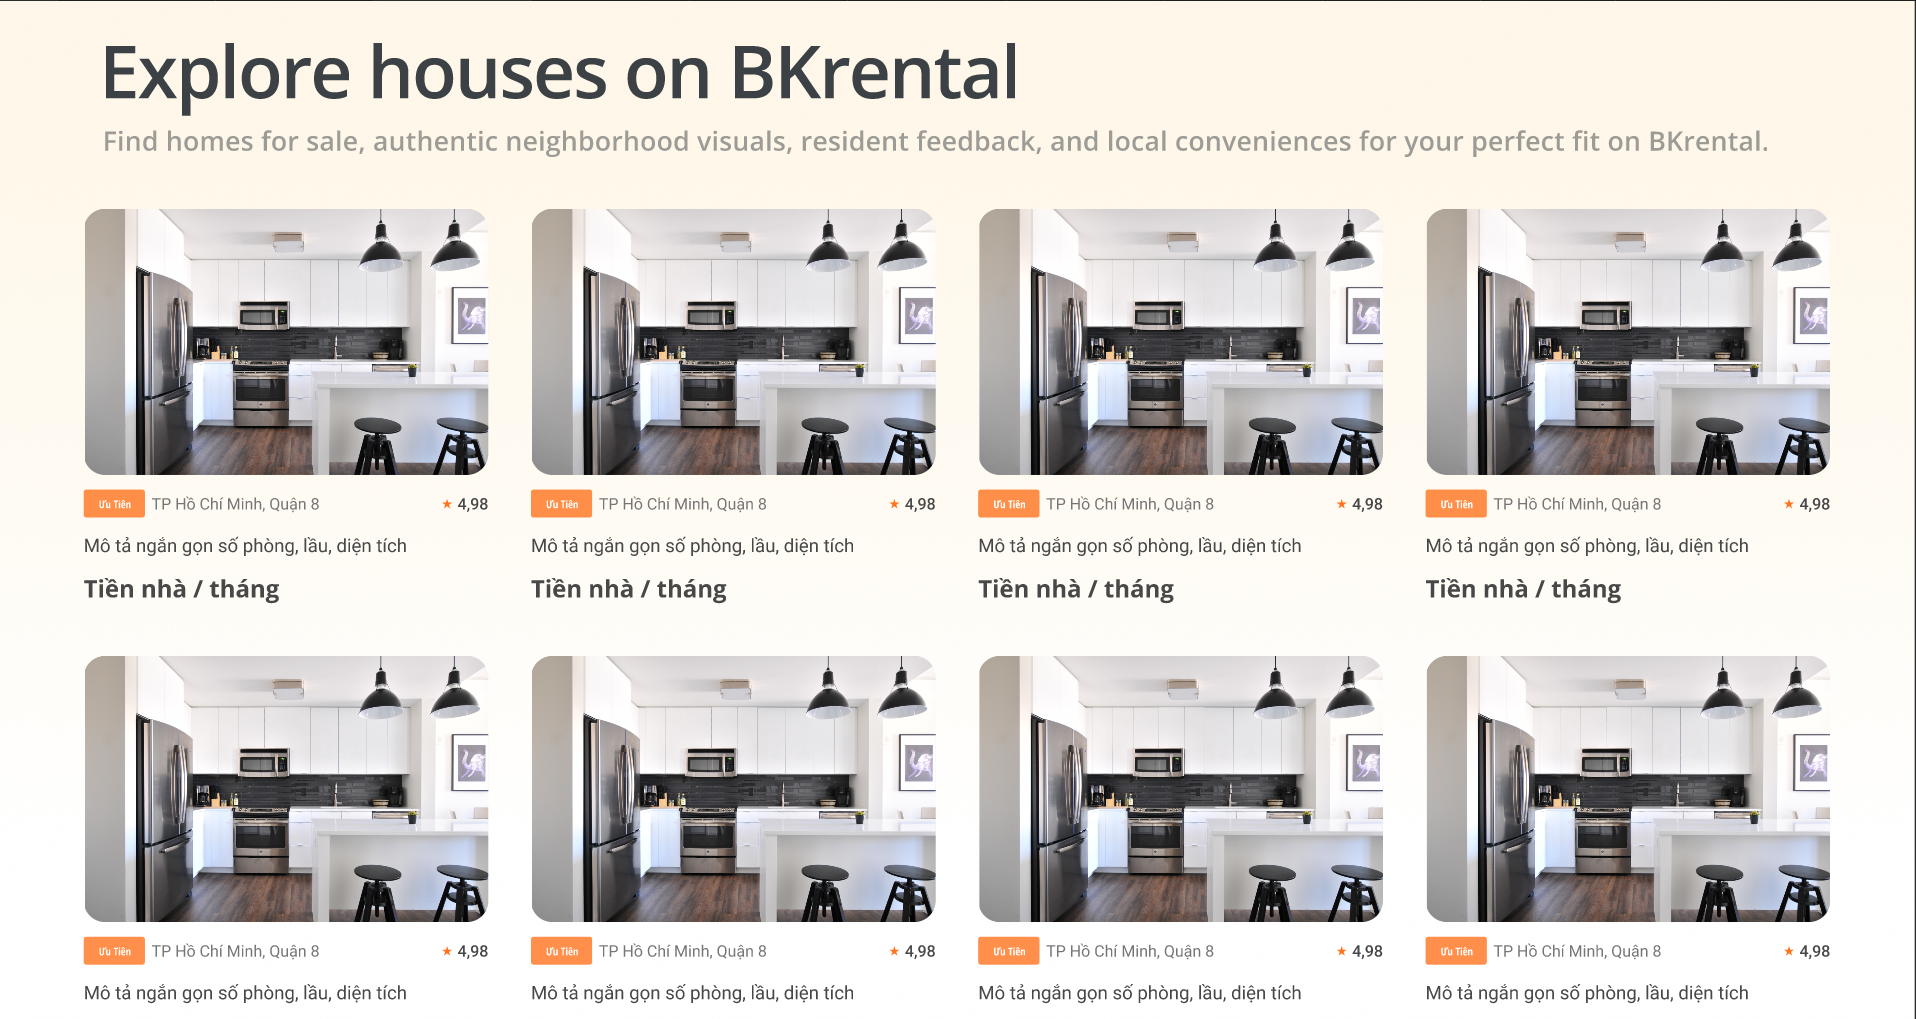
\includegraphics[width=0.8\textwidth]{Images/Mockup/rental_posts.png}
    \caption{The list of rental posts}
    \label{fig:rental-posts} 
\end{figure}

When the user clicks on a rental post, the rental detail page will be displayed. The rental detail page contains the information of the rental post such as the name, address, price, area, description, owner name, owner contact, post date, and the link to the original post. The rental detail page is shown in Figures \ref{fig:rental-detail-page} and \ref{fig:rental-detail-page-2}

\begin{figure}[ht]
    \centering
    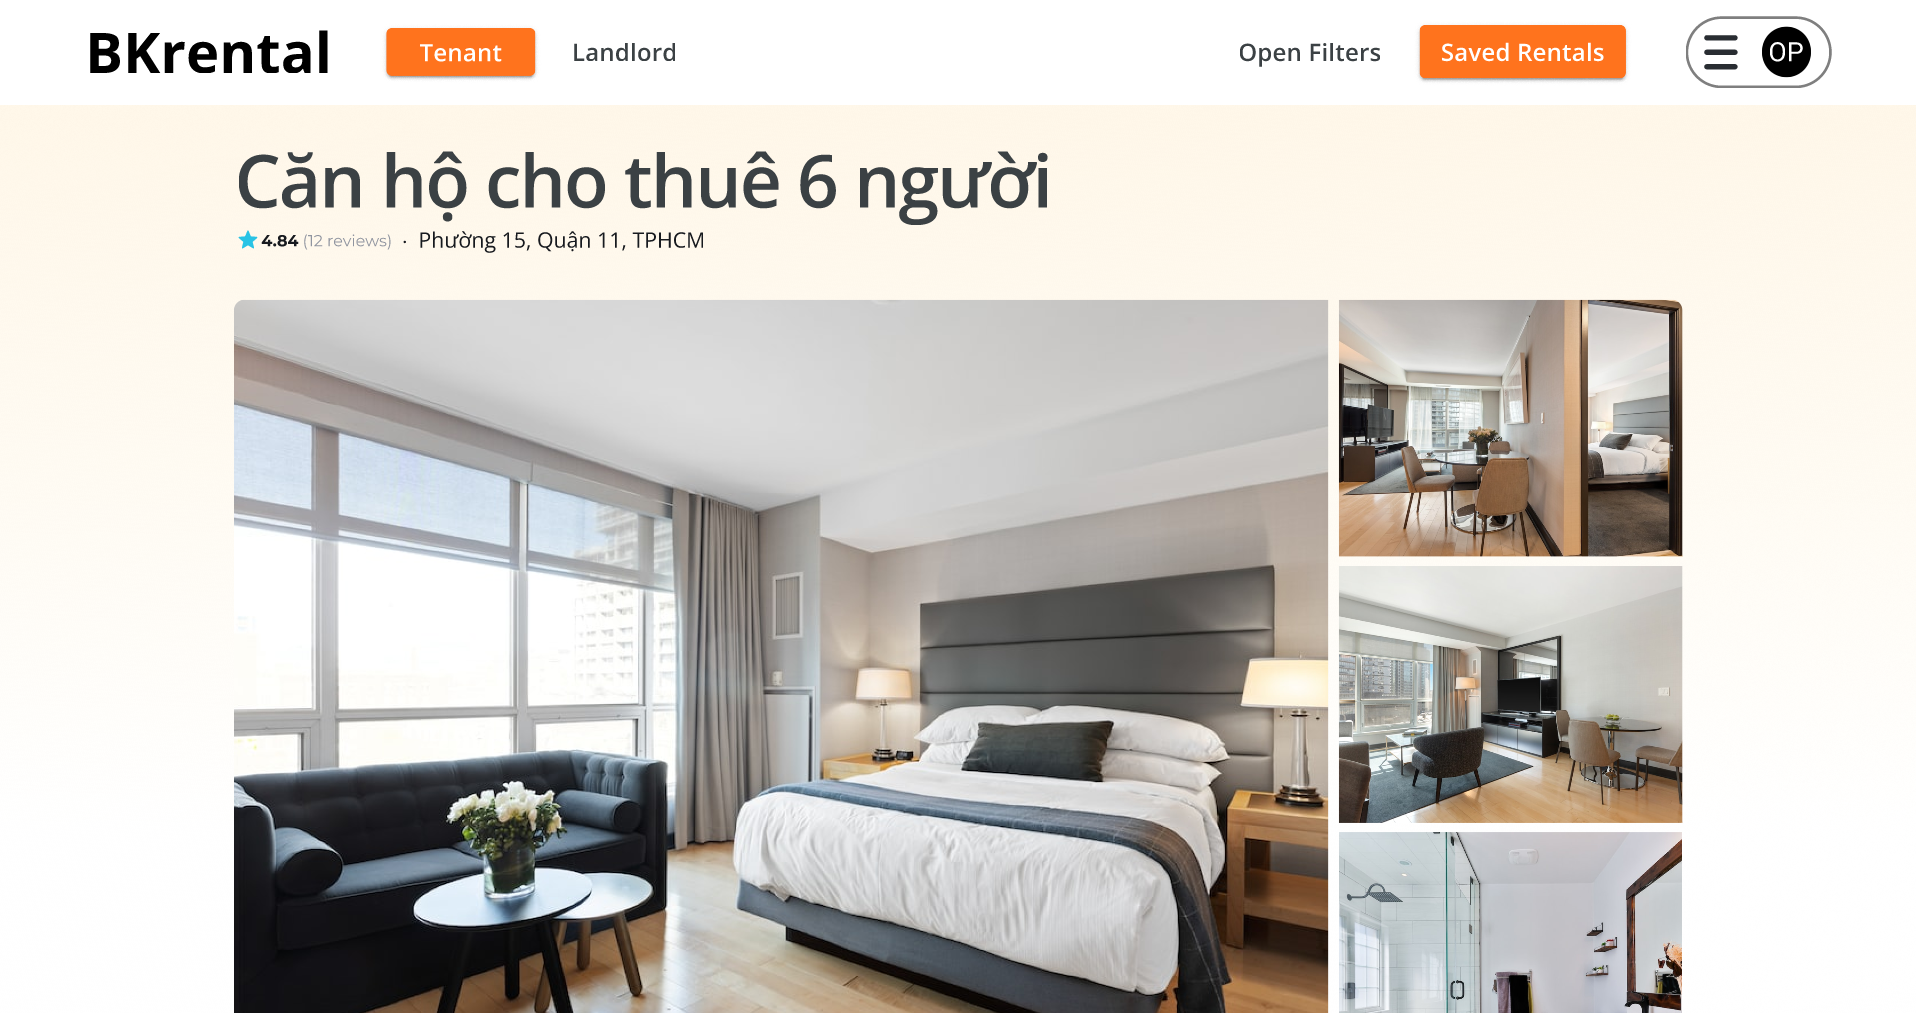
\includegraphics[width=\textwidth]{Images/Mockup/rental_detail_1.png}
    \caption{The rental detail page}
    \label{fig:rental-detail-page}
\end{figure}

\begin{figure}[ht]
    \centering
    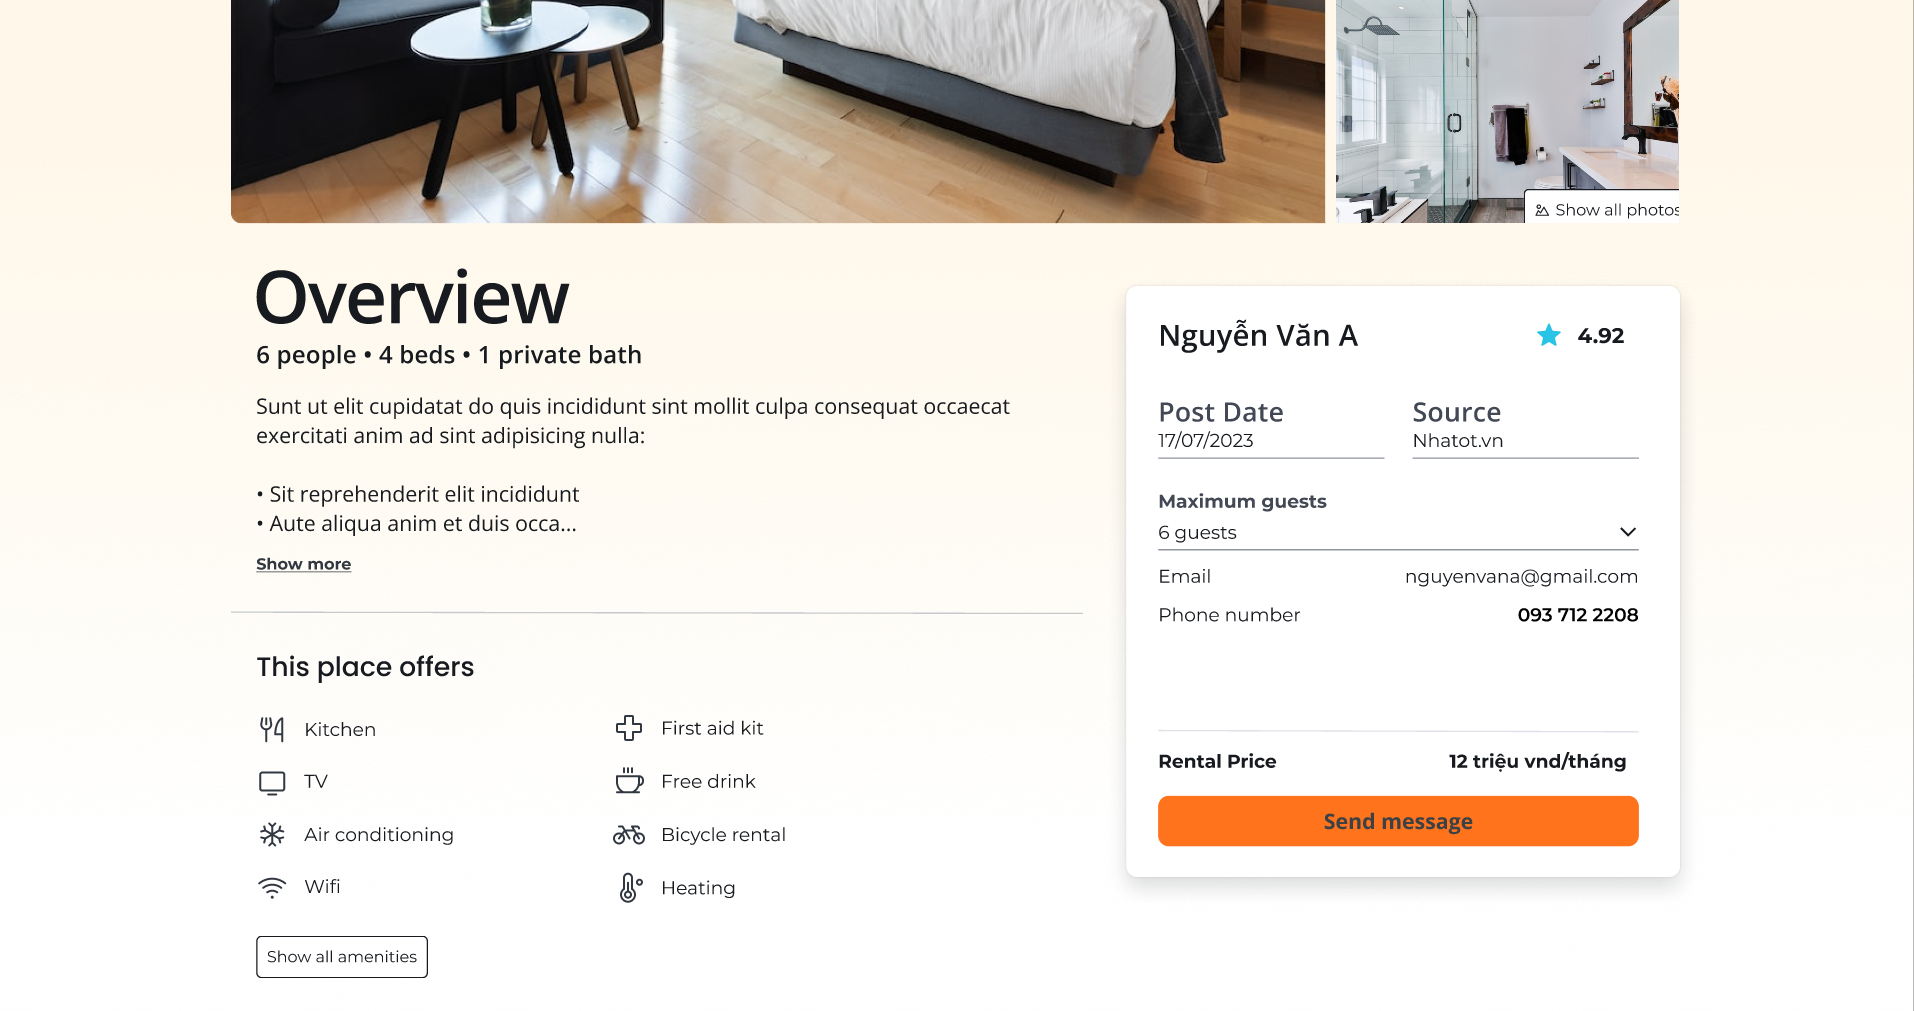
\includegraphics[width=\textwidth]{Images/Mockup/rental_detail_2.png}
    \caption{The rental detail page (continue)}
    \label{fig:rental-detail-page-2}
\end{figure}
\clearpage

\subsubsection{Search and Filter page}
Our website allows the user to search by keyword and filter the rental posts by some criteria such as property type, price range, number of rooms, number of beds, area and amenities. 

\begin{figure}[ht]
    \centering
    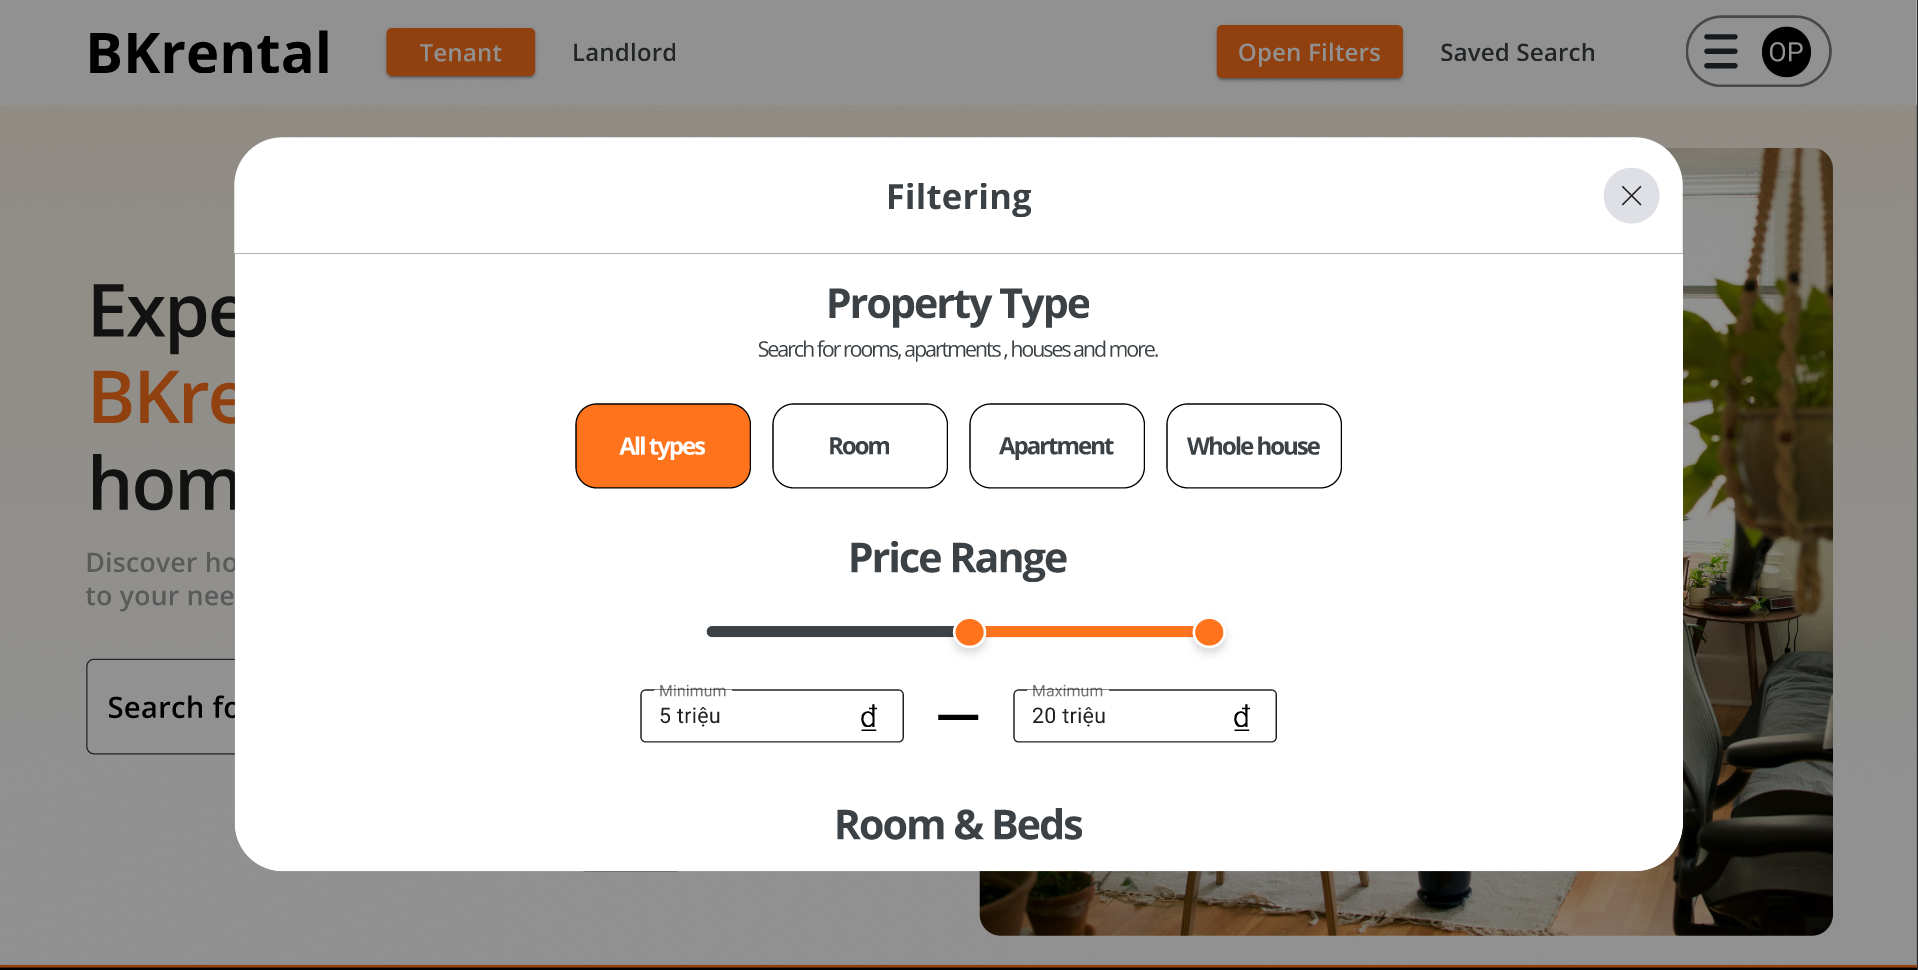
\includegraphics[width=\textwidth]{Images/Mockup/rental_filter_1.png}
    \caption{The rental filter page}
    \label{fig:rental-filter-1} 
\end{figure}

\begin{figure}[ht]
    \centering
    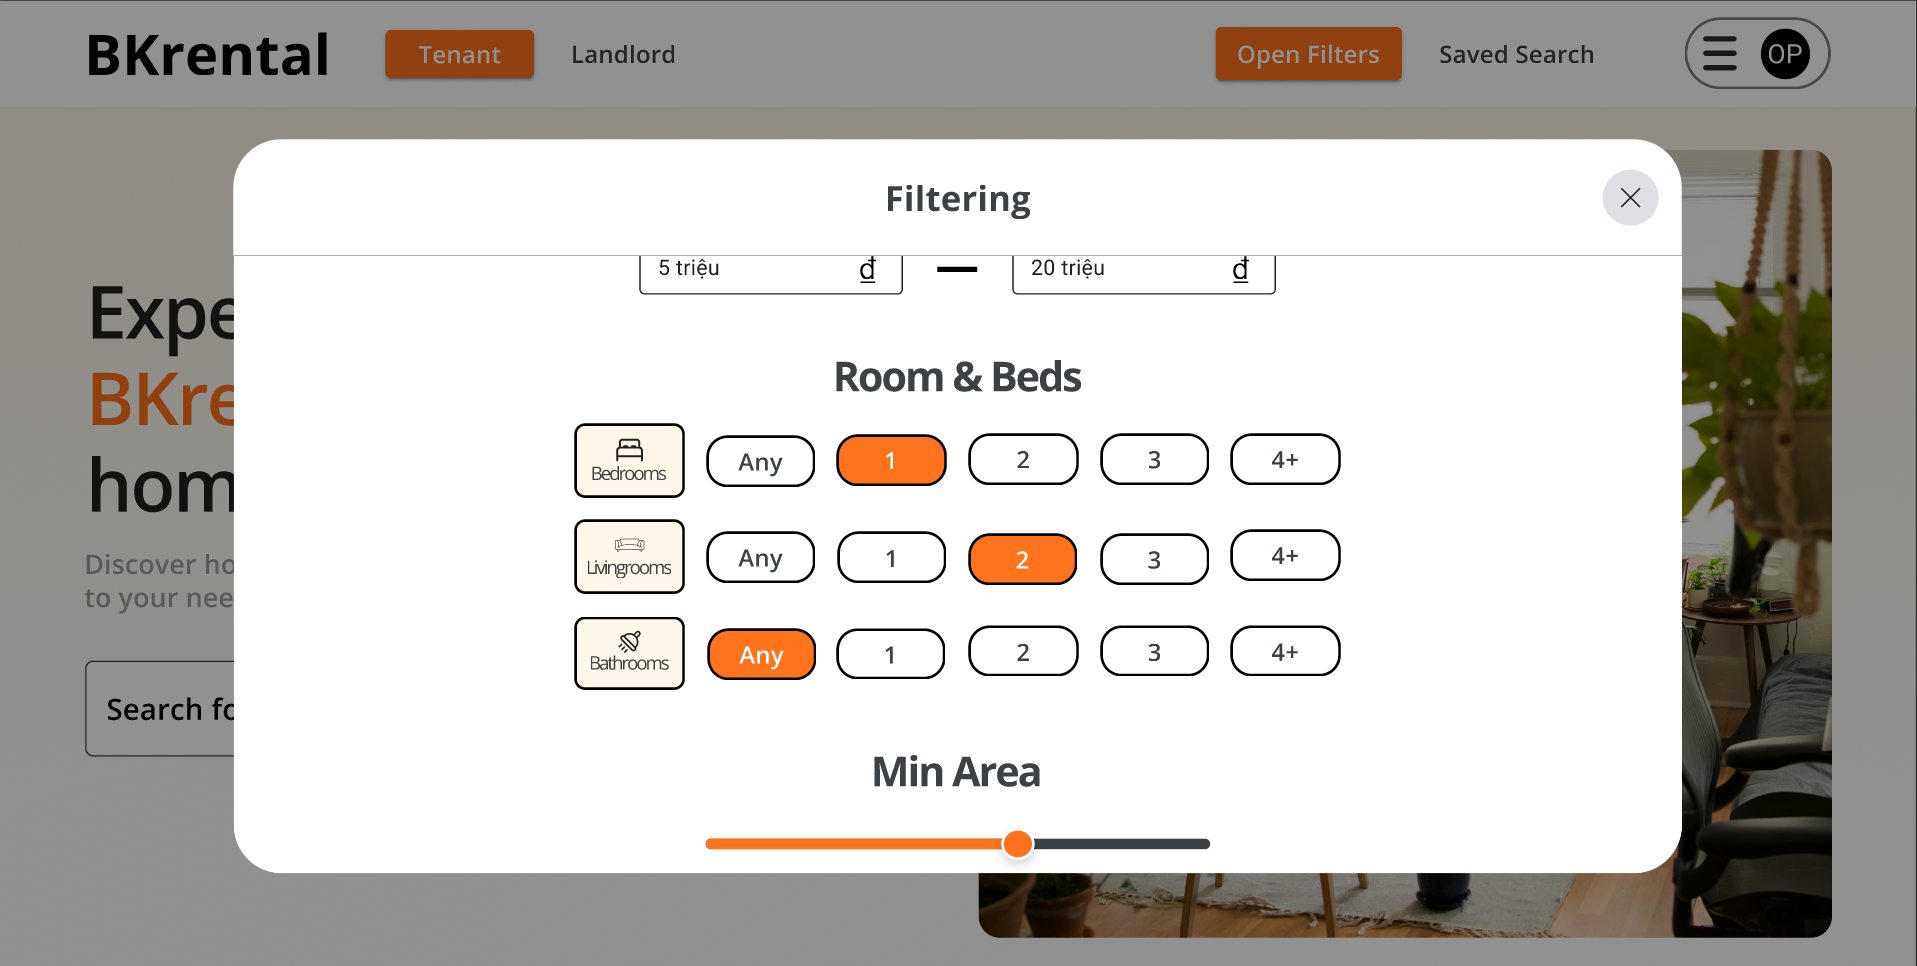
\includegraphics[width=\textwidth]{Images/Mockup/rental_filter_2.png}
    \caption{The rental filter page (continue)}
    \label{fig:rental-filter-2} 
\end{figure}

\begin{figure}[ht]
    \centering
    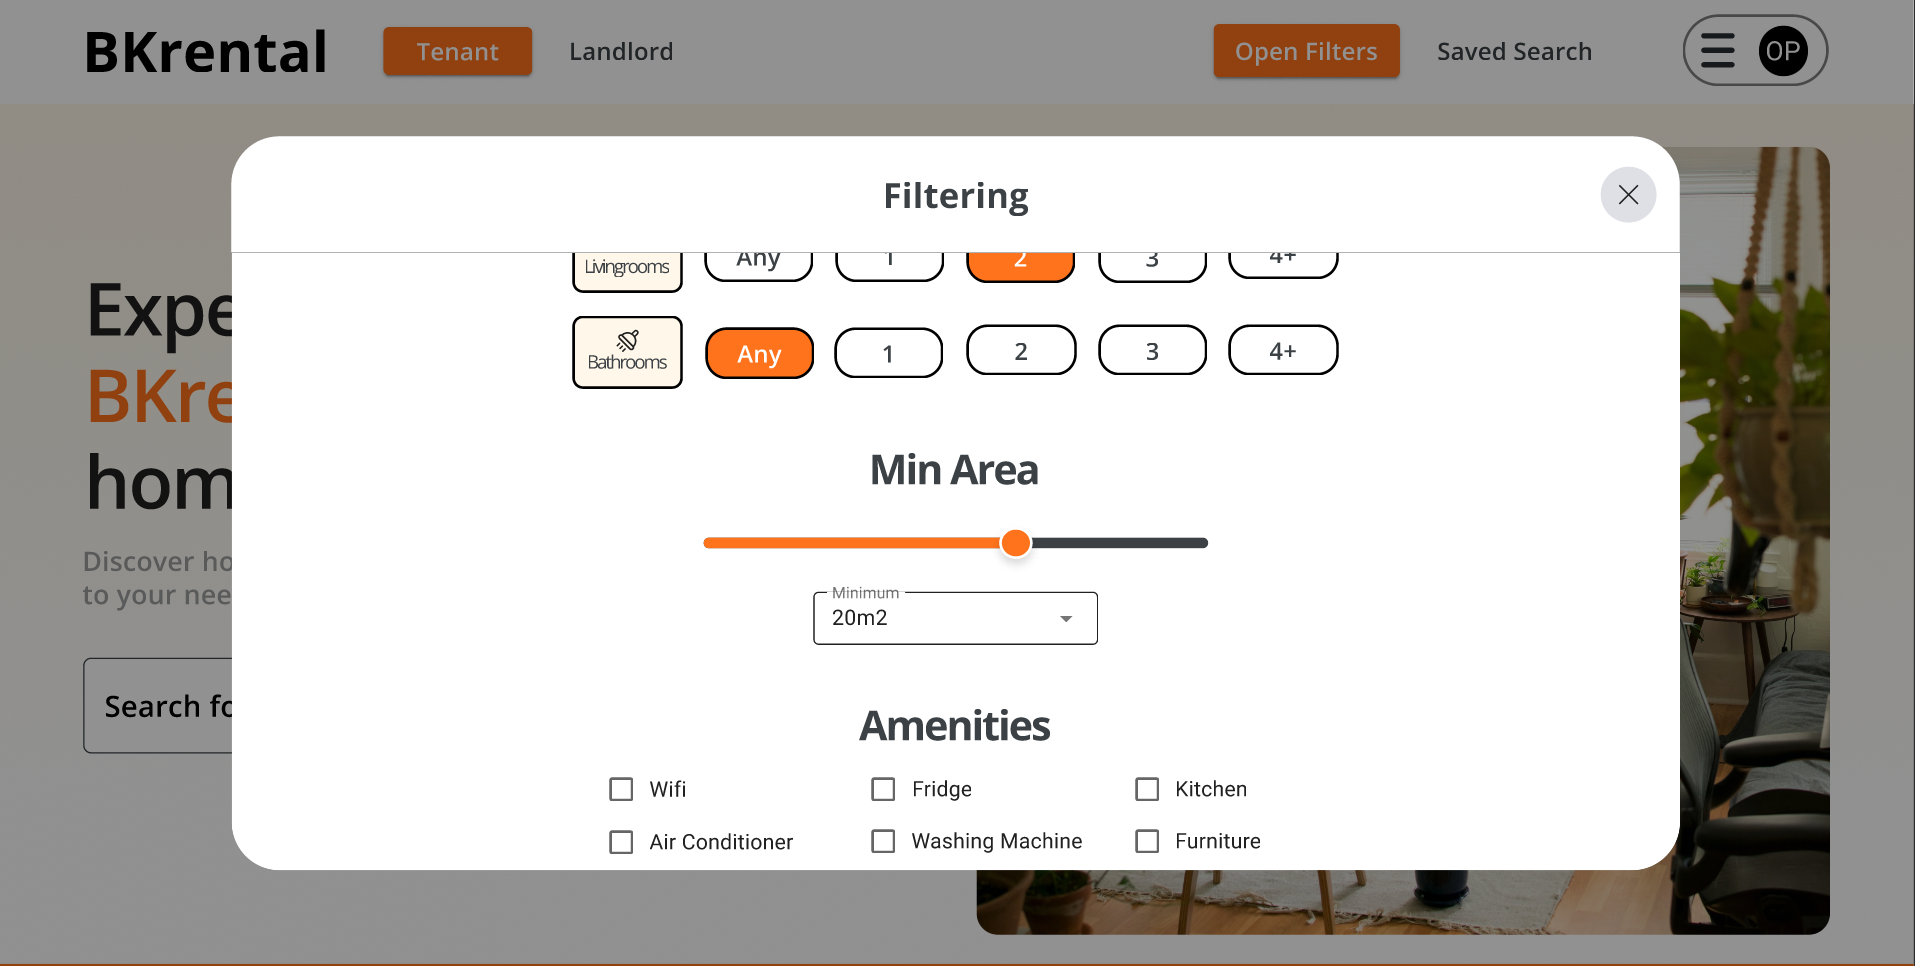
\includegraphics[width=\textwidth]{Images/Mockup/rental_filter_3.png}
    \caption{The rental filter page (continue)}
    \label{fig:rental-filter-3} 
\end{figure}

\clearpage

\subsubsection{Chatbot interface}

\begin{figure}[ht]
    \centering
    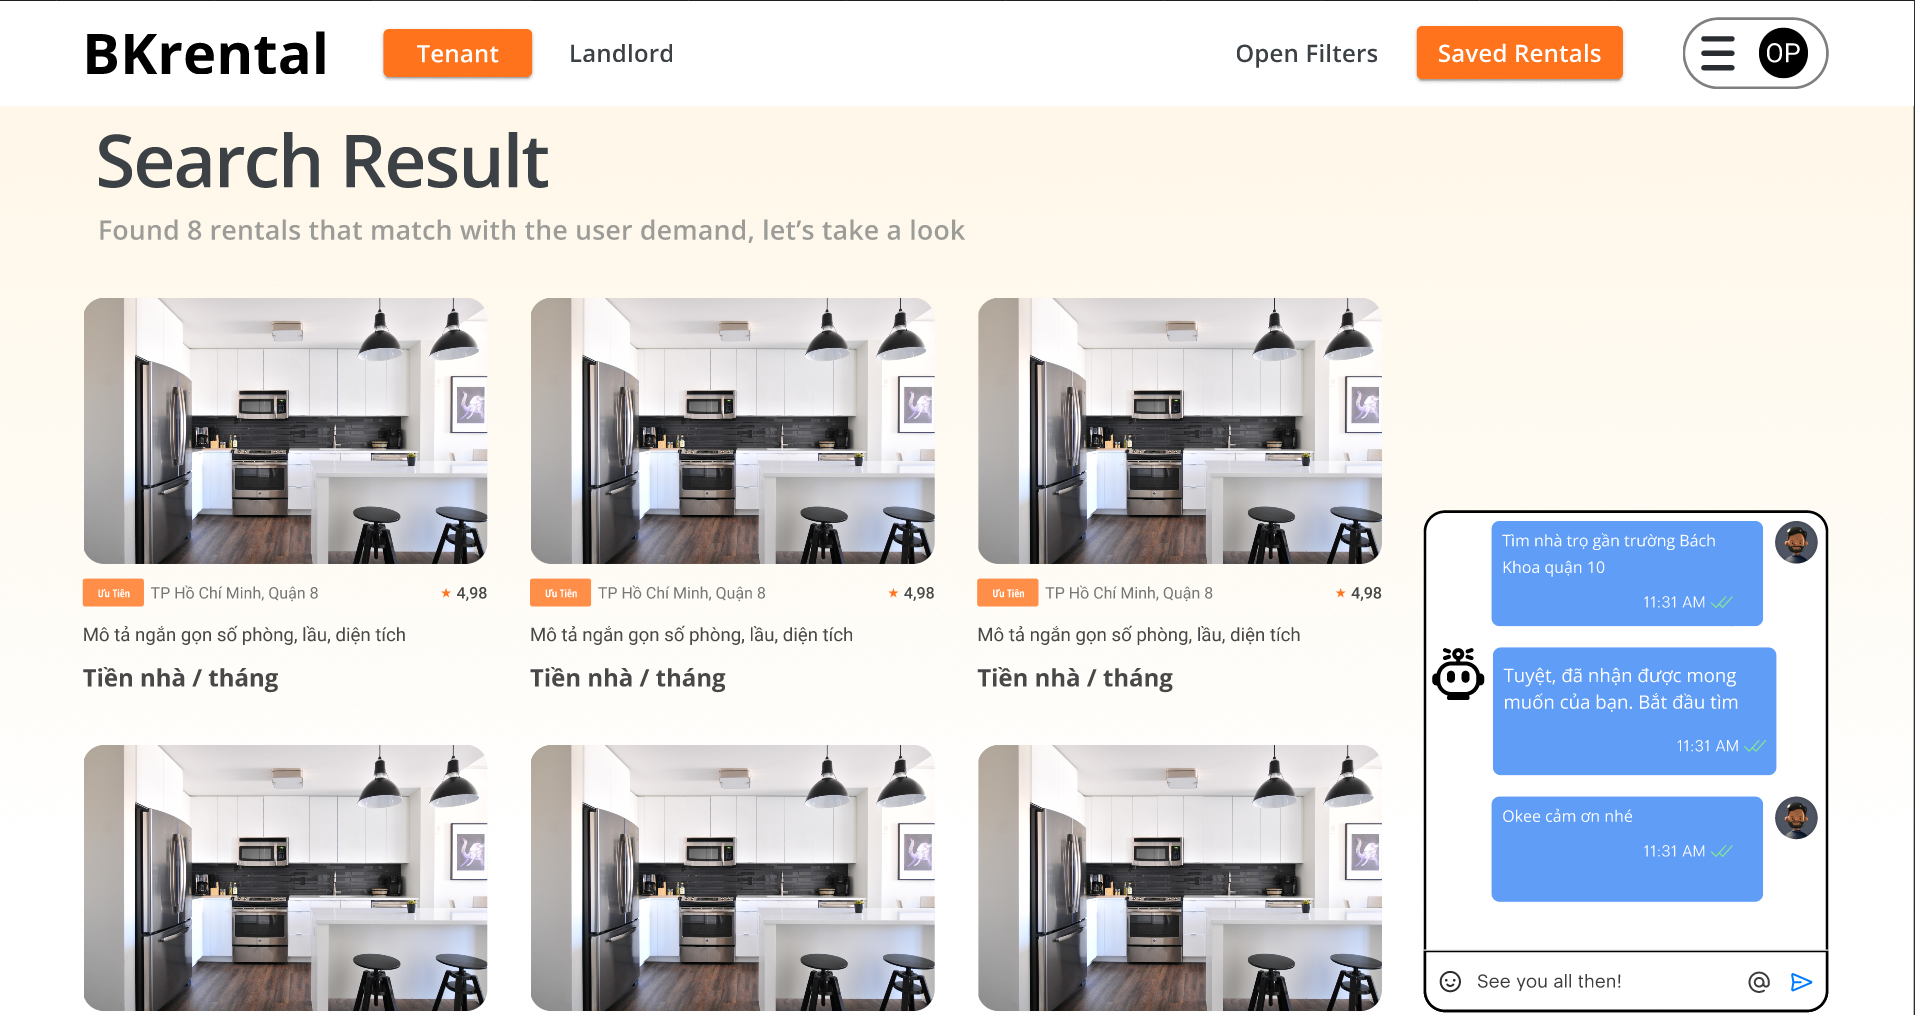
\includegraphics[width=\textwidth]{Images/Mockup/chatbot.png}
    \caption{The chatbot interface}
    \label{fig:chatbot}
\end{figure}

\clearpage

\subsubsection{Landlord pages}
We have landlord pages that allow the landlord to post their rental information and manage their property. Figures \ref{fig:create-rental-1} and \ref{fig:create-rental-2} show the form for the landlord to create a new rental post

\begin{figure}[ht]
    \centering
    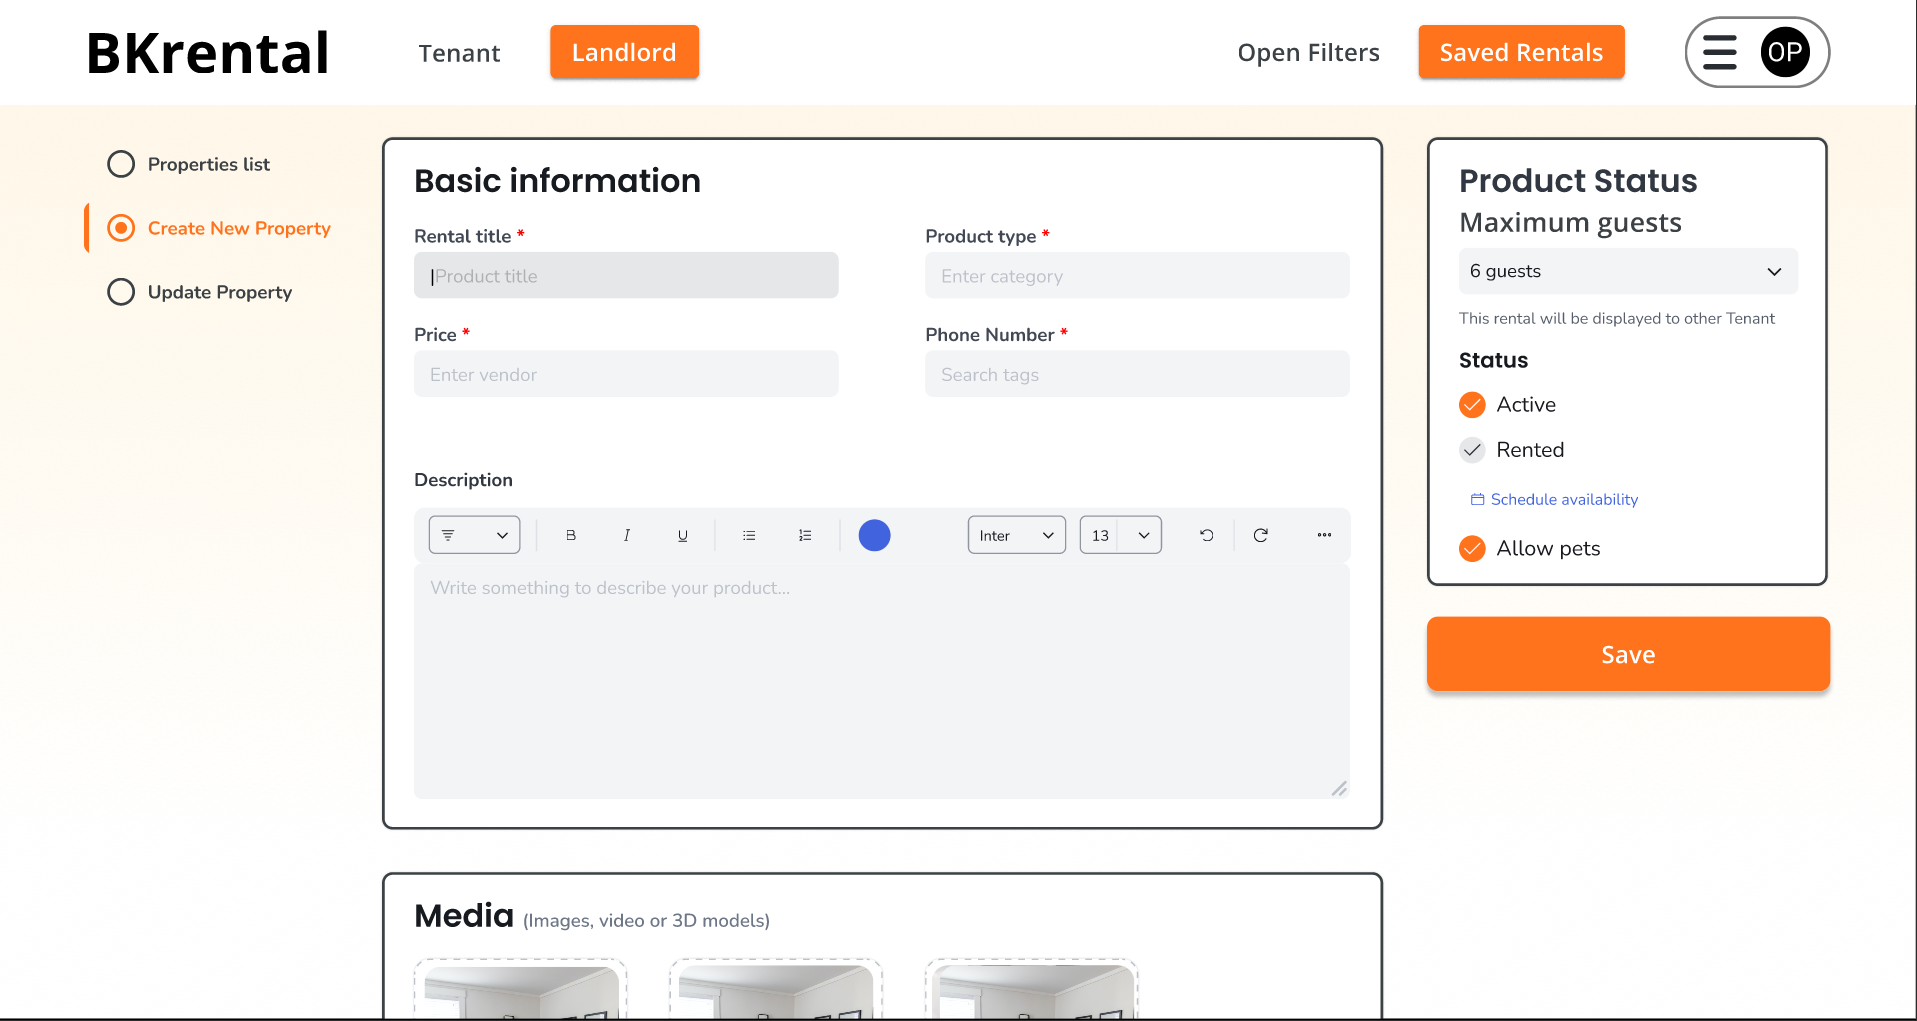
\includegraphics[width=0.8\textwidth]{Images/Mockup/create_rental_1.png}
    \caption{The form for the landlord to create a new rental post}
    \label{fig:create-rental-1}
\end{figure}

\begin{figure}[ht]
    \centering
    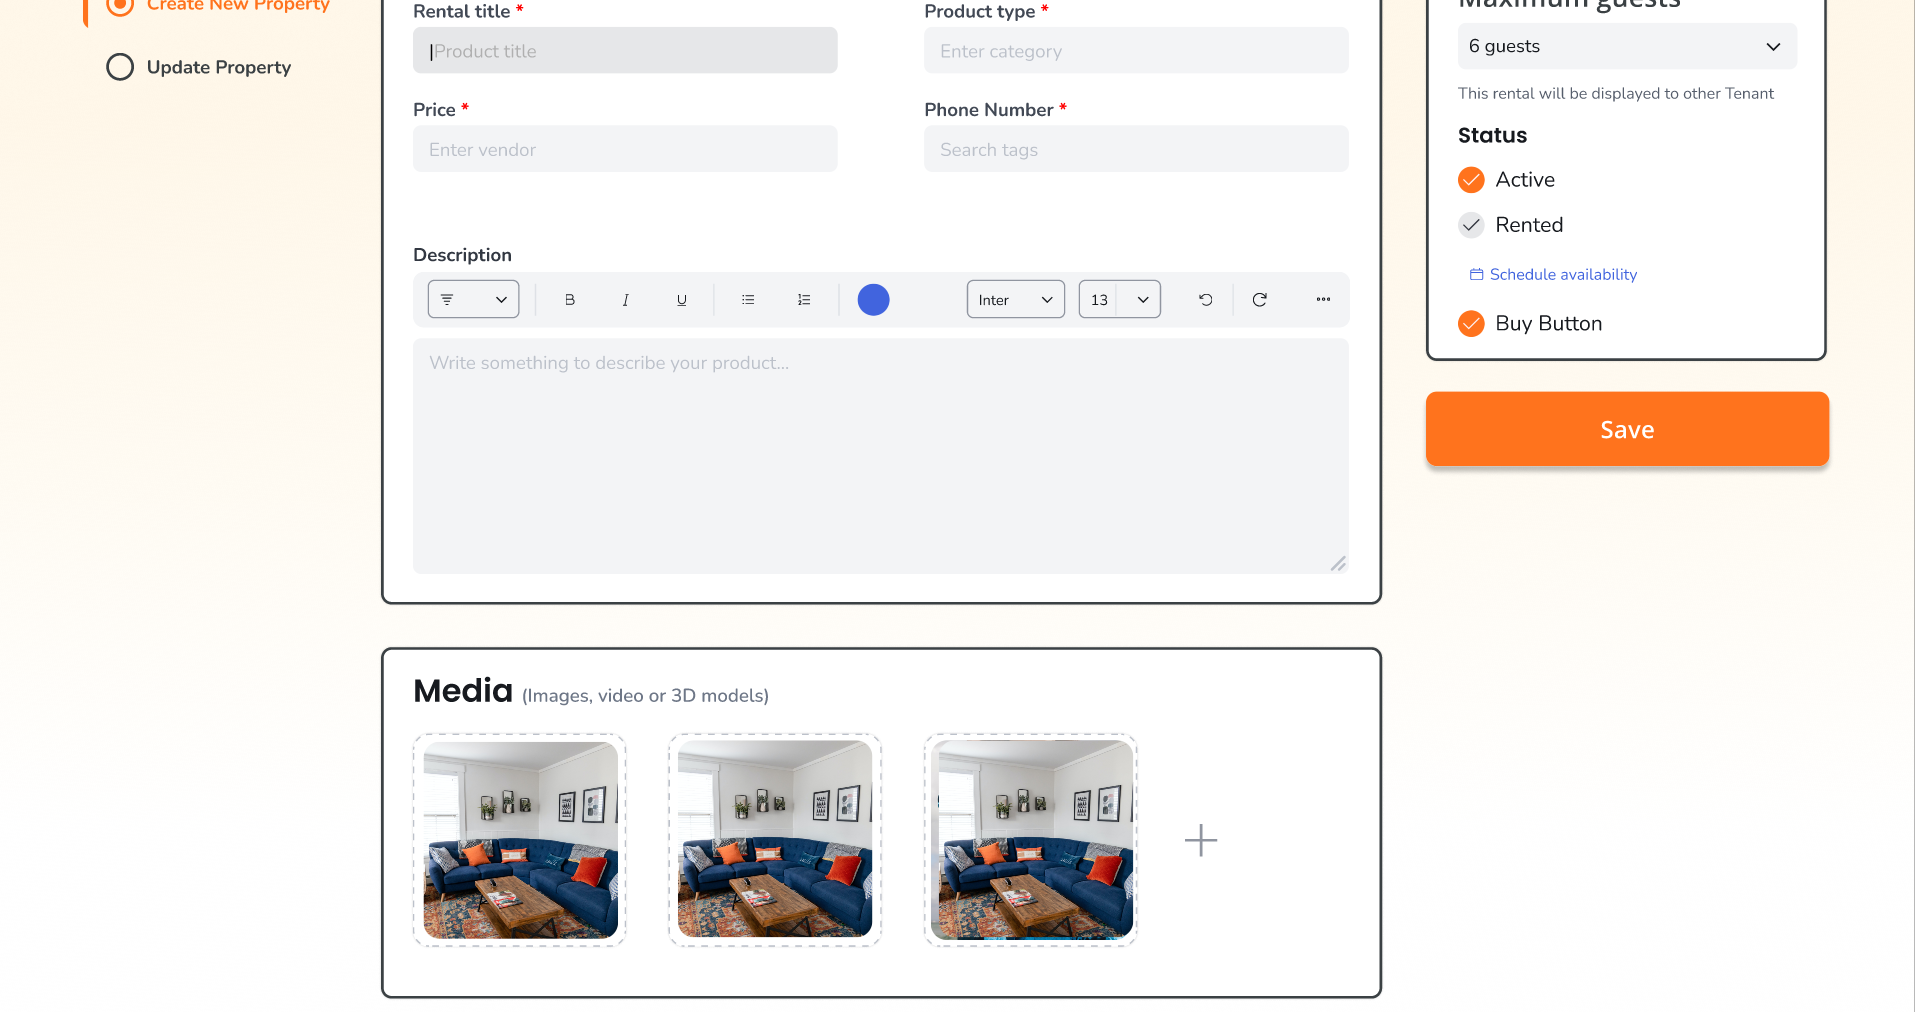
\includegraphics[width=0.8\textwidth]{Images/Mockup/create_rental_2.png}
    \caption{The form for the landlord to create a new rental post (continue)}
    \label{fig:create-rental-2}
\end{figure}

\clearpage

\begin{figure}[ht]
    \centering
    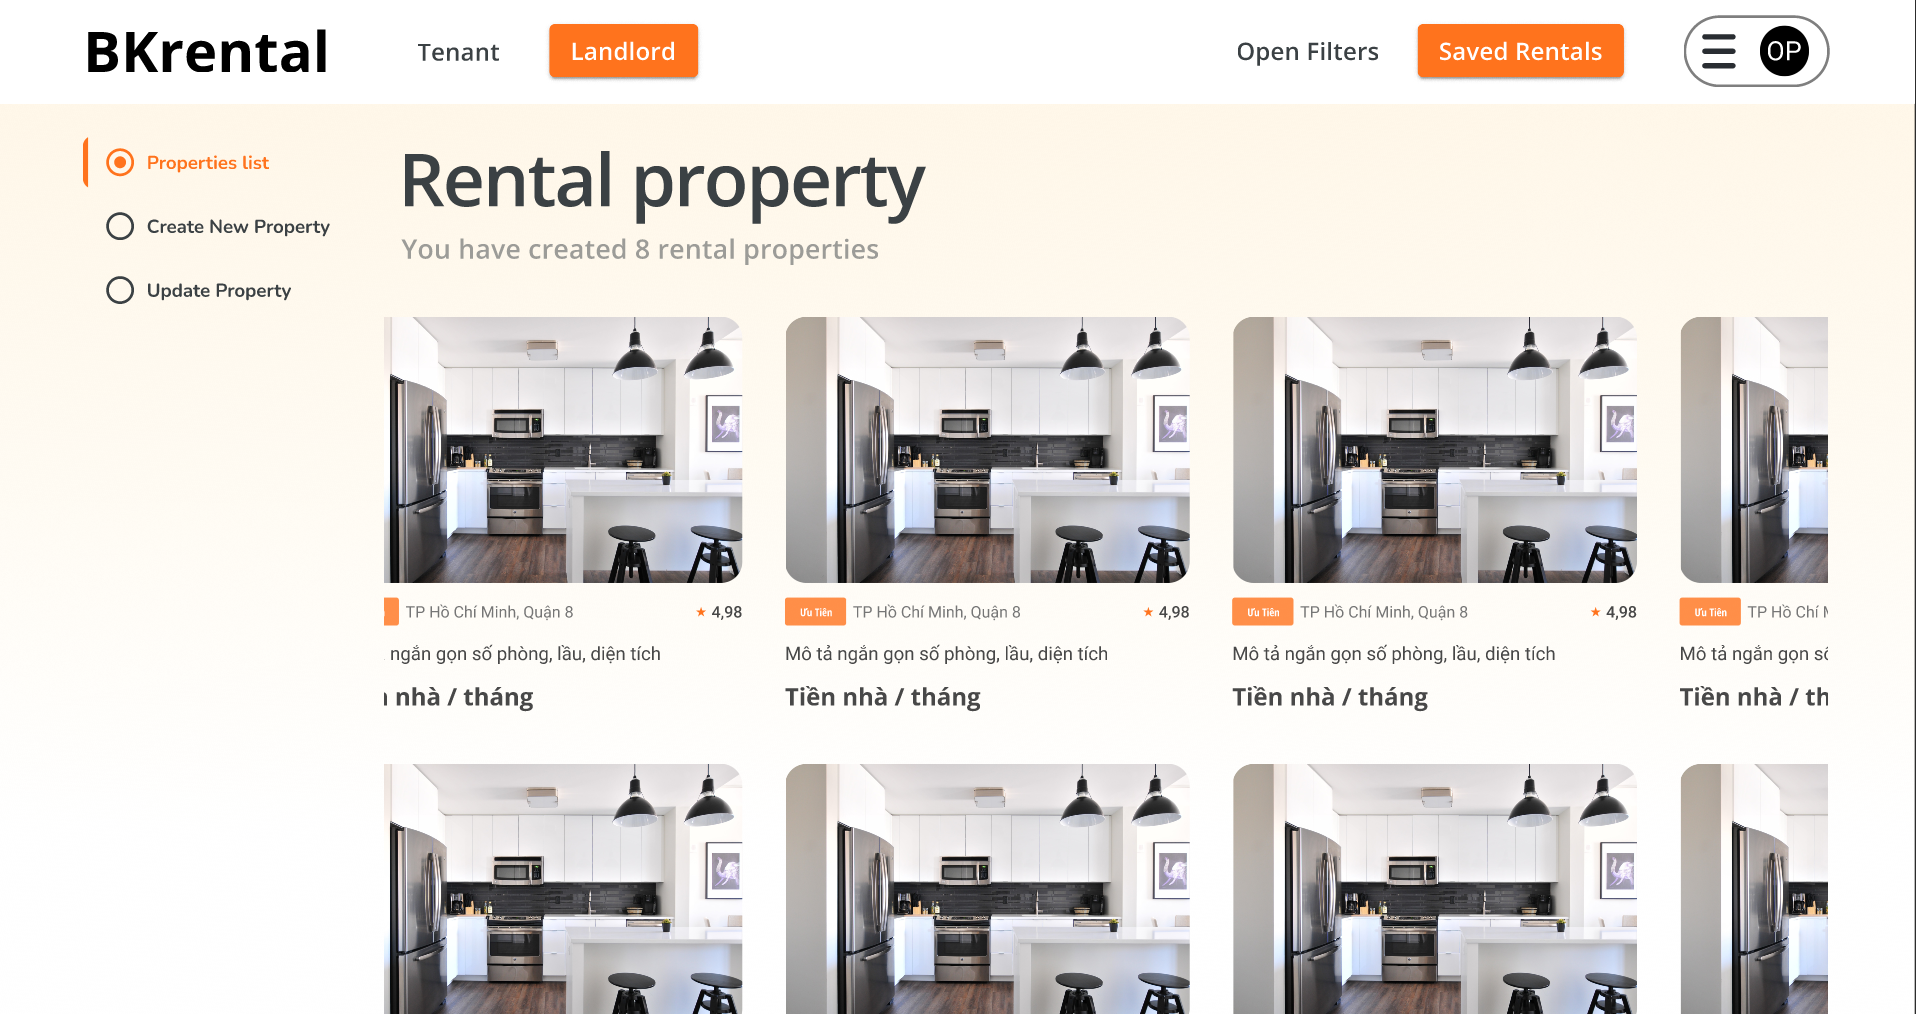
\includegraphics[width=0.8\textwidth]{Images/Mockup/property_list.png}
    \caption{The list of Landlords' properties}
    \label{fig:property_list}
\end{figure}

\begin{figure}[ht]
    \centering
    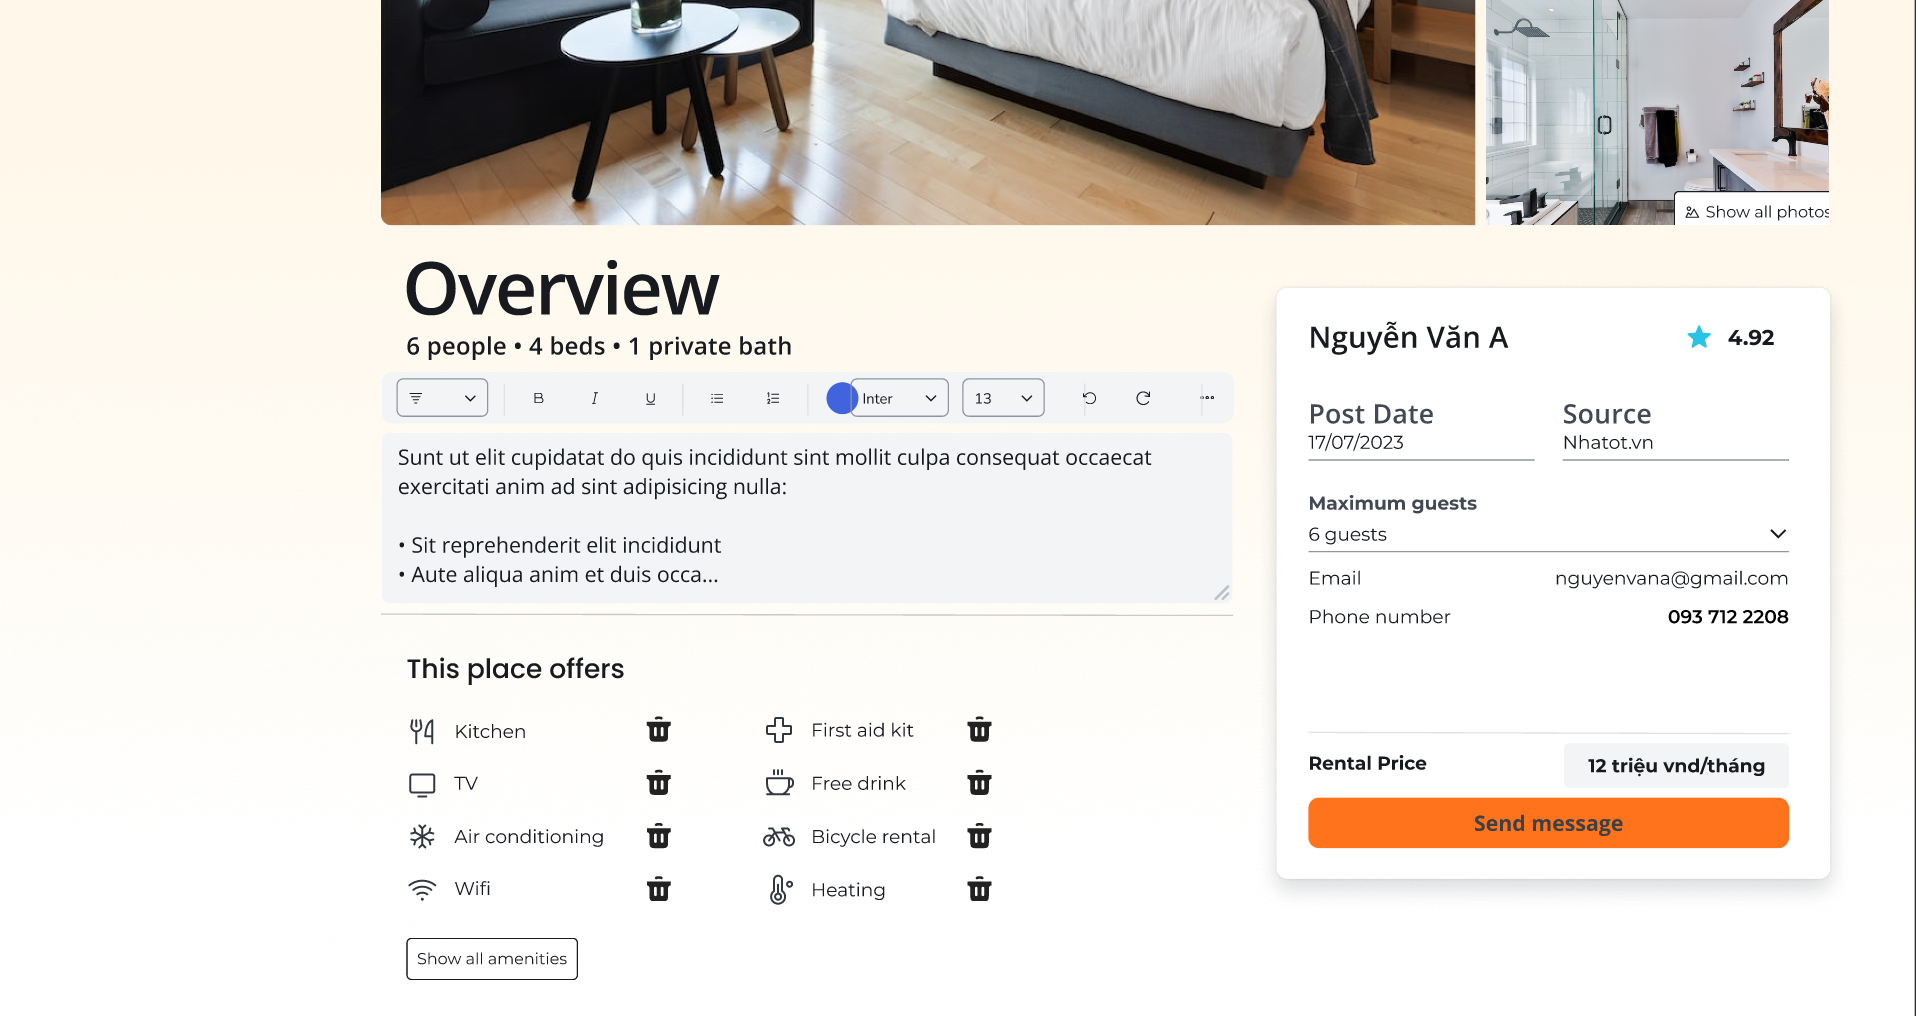
\includegraphics[width=0.8\textwidth]{Images/Mockup/update_rental.png}
    \caption{The form for the landlord to update a rental post}
    \label{fig:update_rental}
\end{figure}

\clearpage

\subsection{Crawler service}

\subsubsection{The Facebook Crawler}
We developed a tool that receives the list of Facebook pages and group URLs as input. Then this tool will get all the posts from these pages and groups and store them in the output file. The tool is implemented using NodeJS and the Puppeteer library.

We chose the list of 40 Facebook pages and groups in the real estate domain, especially the ones that have the most interactions. The list of these pages and groups is stored in the input file. The sample of the input file is shown in Figure \ref{fig:facebook-crawler-input}.

\begin{figure}[ht]
    \centering
    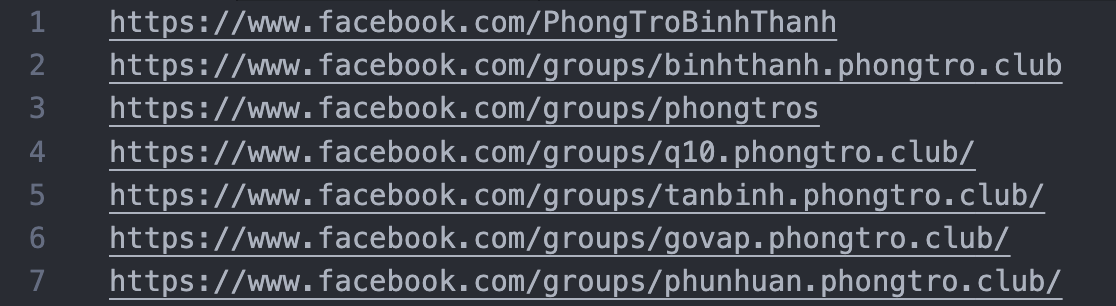
\includegraphics[width=0.8\textwidth]{Images/9.Implementation/facebook_crawler_input.png}
    \caption{The sample input of the Facebook crawler}
    \label{fig:facebook-crawler-input}
\end{figure}

When running the tool, the tool will read the input file and get the list of Facebook pages and groups. Then it will open a new browser window and log in to Facebook. After that, it will visit each page and group in the list and get all the posts from these pages and groups. Finally, it will store the posts in the output file. The output file is a text file that contains the list of posts in text format. Each post is separated by a new line character. After the tool finishes crawling all the posts, we get the output file that contains nearly \textbf{2000 posts}. The sample output of the tool is shown in Figure \ref{fig:facebook-crawler}.

\begin{figure}[ht]
    \centering
    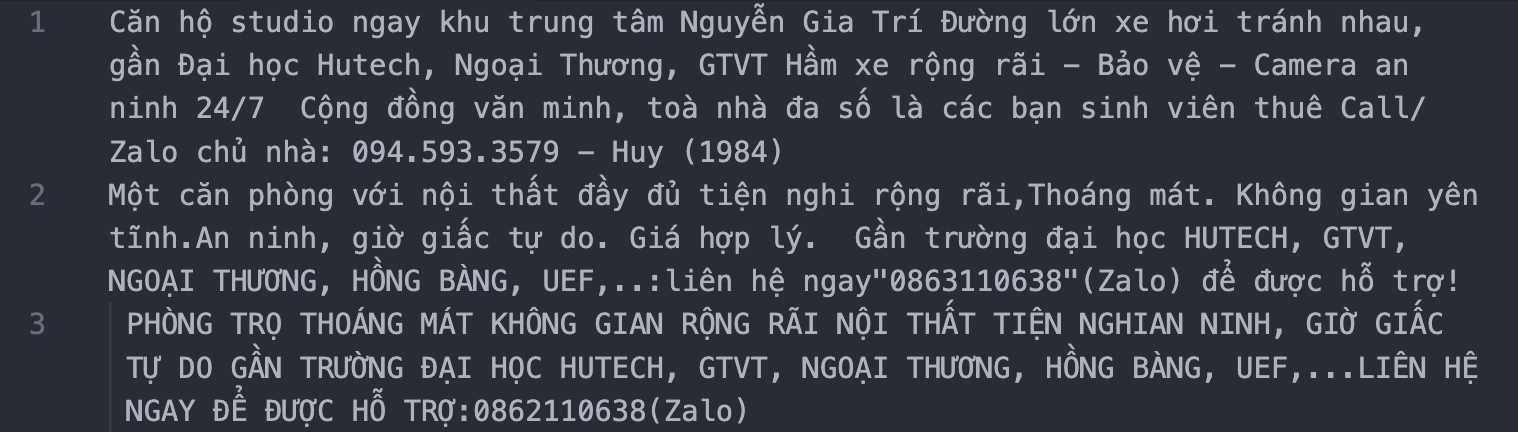
\includegraphics[width=0.8\textwidth]{Images/9.Implementation/facebook_crawler_output.png}
    \caption{The sample output of the Facebook crawler}
    \label{fig:facebook-crawler}
\end{figure}

\subsubsection{The Real Estate Website Crawler}
We also developed a tool that crawls the data from some popular real estate websites in Vietnam such as mogi.vn. The tool is implemented using Python and Scrapy. Because these websites are server-side rendered websites, we can take advantage of the Scrapy library to crawl the data. 

From the website link, we developed a Spider Scrapy. The main role of the Spider is downloading the content of the website parsing the content and getting the data by using CSS selector. The sample code of the parser is shown below

\begin{lstlisting}[language=Python]
def parse_detail_info(self, response):
    general_info = response.css('div.main-info')
    main_info = response.css('div.info-attrs.clearfix > *')
    agent_name_link = response.css('div.agent-name::text').get()
    agent_name_no_link = response.css('div.agent-name a::text').get()
    agent_name = agent_name_link if agent_name_link else agent_name_no_link

    yield rental_item = {
        'name': general_info.css('div.title h1::text').get(),
        'address': general_info.css('div.address::text').get(),
        'price': general_info.css('div.price::text').get(),
        'area': main_info[0].css('span:nth-of-type(2)::text').get(),
        'description': response.css('div.info-content-body').get(),
        'owner_name': agent_name,
        'owner_contact': response.css('div.agent-contact').get(),
        'post_date': main_info[2].css('span:nth-of-type(2)::text').get(),
        'prop_info_url': response.meta.get('prop_info_url')
    }
\end{lstlisting}

After crawling, we got the data in CSV format with \textbf{12288 rows}. Each row is a rental post with the following fields: name, address, price, area, description, owner name, owner contact, post date, and the link to the original post. Figure \ref{fig:sample-crawling-data} shows the sample data returned by the crawler. 

\begin{figure}[ht]
    \centering
    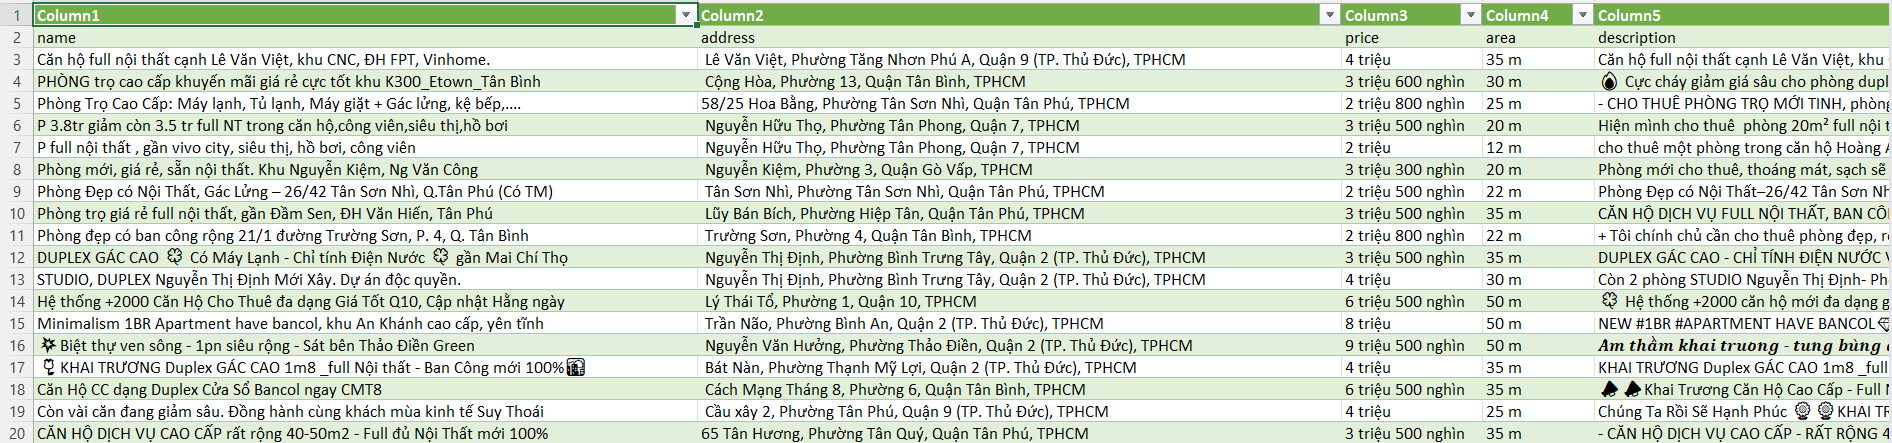
\includegraphics[width=0.8\textwidth]{Images/9.Implementation/sample_crawling_data.png}
    \caption{The sample data returned by the crawler}
    \label{fig:sample-crawling-data}
\end{figure}

The full dataset can be found \href{https://www.kaggle.com/datasets/ef8770394a7256fd4e5270fd4a3692235a620fc85ac18128efd1b44d31aa5b1b}{here}.

\subsection{Intent classification model}
We have implemented the intent classification model as discussed subsection in \ref{sec:intent-classification-model} with Pytorch and PhoBERT library. The model is trained on the dataset containing 1000 labeled messages. We split the dataset into 2 parts: 80\% for training and 20\% for testing. We trained the model for 10 epochs with a batch size of 32. Figure \ref{fig:intent-classification-result} shows the accuracy of the model during the training process. Overall, the model achieves an accuracy of 97.4\% on the training set and 96.5\% on the test set. 

\begin{figure}[ht]
    \centering
    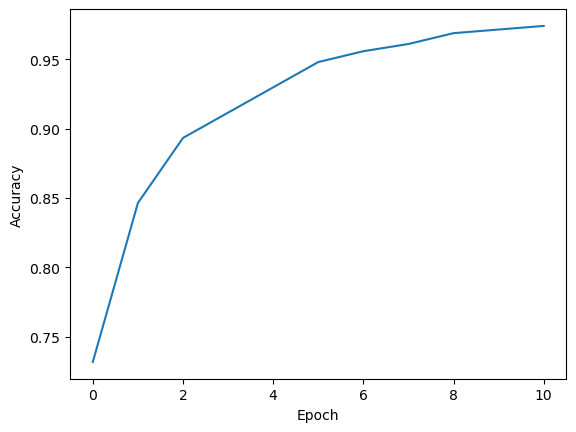
\includegraphics[width=0.7\textwidth]{Images/9.Implementation/intent_classifier_accuracy.png} 
    \caption{The accuracy of the intent classification model during the training process}
    \label{fig:intent-classification-accuracy}
\end{figure}

\begin{figure}[ht]
    \centering
    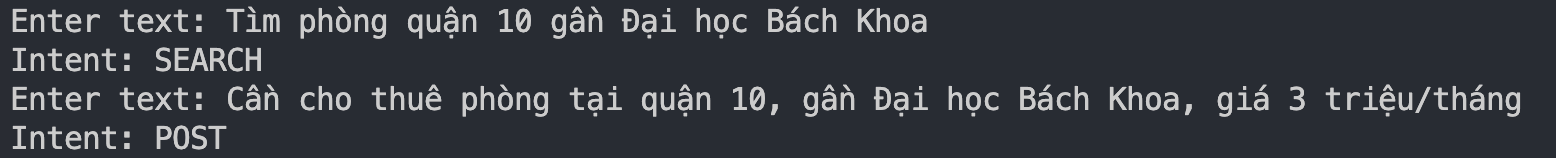
\includegraphics[width=0.8\textwidth]{Images/9.Implementation/intent_classifier_result.png}
    \caption{The sample result of intent classification model}
    \label{fig:intent-classification-result}
\end{figure}


